
\section{Introduction}


% video analytics is coming to age
Video analytics is coming to age.
Modern computer-vision techniques, in the form of deep convolutional 
neural networks (\nn), are set to transform our life by automating 
large-scale analytics of video data that so far has relied on 
human-based inspection.
Indeed, many organizations~\cite{??,??} have piloted \nn-based 
analytics on thousands of video feeds from traffic cameras, dash 
cams, and drones on a 24$\times$7 basis.
This trend is fueled by intensive on-going research~\cite{??,??}
from the vision community constantly improving the inference accuracy 
by ever more complex \nn solutions.

% finding good config is the key to optimizing cost-accuracy tradeoff
Unfortunately, applying \nn to video data at scale can be prohibitively
{\em expensive}.
For instance, one needs a \$9K GPU or \$800/month cloud VM to run
an \nn model~\cite{??} on just a single live video feed with relatively 
low quality, e.g., 720p and 30fps (frames per second). 
Worse still, recent vision techniques have largely improved inference
accuracy at the expense of increased processing time and resource 
consumption~\cite{??}.
Such cost is clearly untenable, and therefore, any practical system 
for video analytics must strike a balance between {\em resource 
consumption} and {\em accuracy}.


\begin{figure}[t!]
\centering
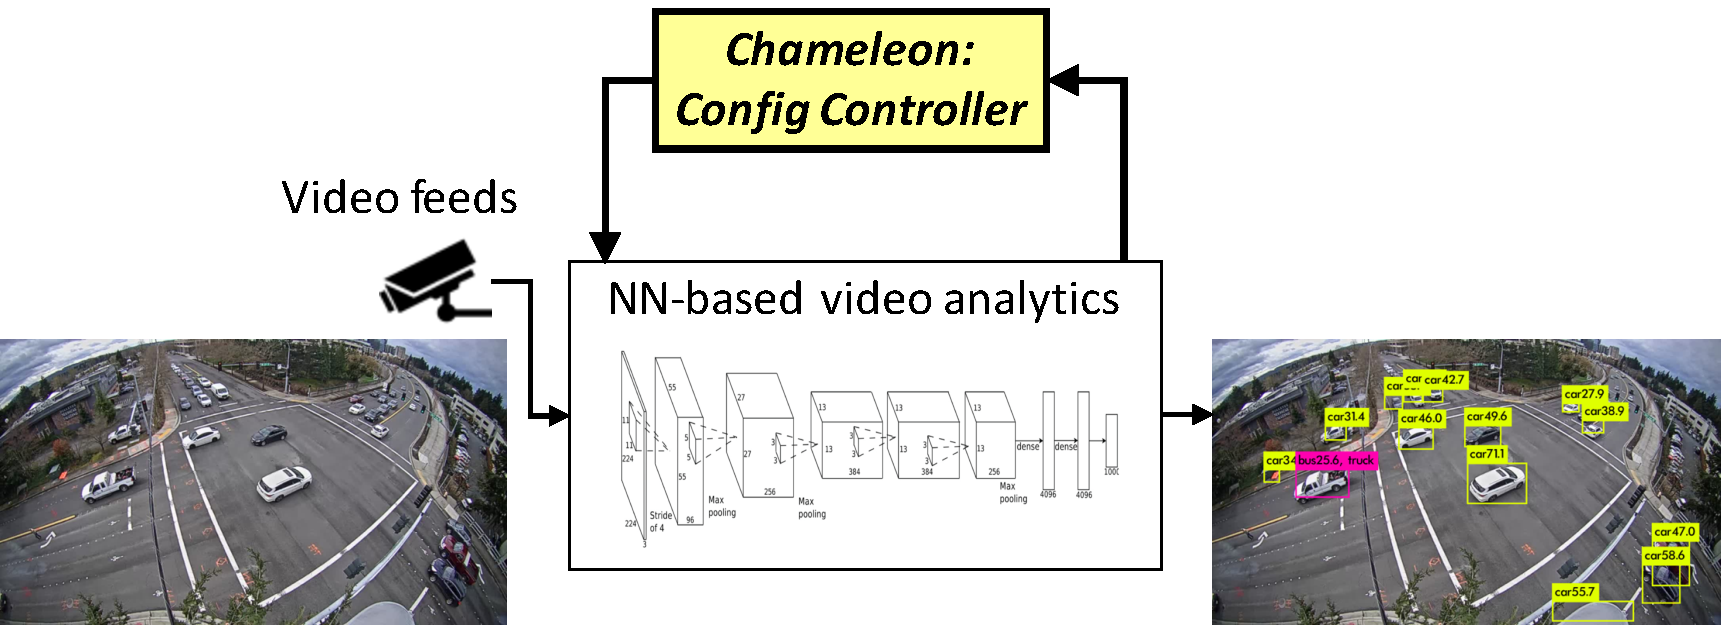
\includegraphics[width=0.5\textwidth]{PaperFigures/Overall.pdf}
\vspace{-0.3cm}
\tightcaption{Overview of \name, which features the configuration 
controller that continuously profiles and dynamically adapts the
\nn configurations.}
\label{fig:overall}
\end{figure}

We present {\em \name}, a video analytics controller, that optimizes 
resource consumption and inference accuracy of existing video 
analytics pipelines by adapting key \nn configurations in real-time.
(Figure~\ref{fig:overall}).
Prior work has observed that it is possible to reduce resource 
consumption with little cost in accuracy by using a cheaper \nn 
configuration (e.g., lower frame rate, resolution, and simplified
inference model)~\cite{videostorm,noscope}.
However, to realize the full potential of tuning the \nn configurations,
the system must cope with the {\em intrinsic variability, both spatial
and temporal, in the resource-accuracy tradeoffs of \nn configurations}.
% The optimal configuration is sensitive to several characteristics
% that varies substantially over time and across video feeds.
For instance, any change in velocity of moving objects can alter
the optimal \nn configuration;
e.g., tracking cars within 5 meters at 30m/s (e.g., highway or 
off-peak hours) requires a frame rate of 6fps, but if cars are at 5m/s 
(e.g., crossroads or traffic jam), 1fps would suffice, 
an 84\% save in computing resources.
Many other factors, e.g., types and sizes of objects,
can similarly affect the resource-accuracy tradeoffs.
% In short, a flexible pipeline that self-adapts in realtime could 
% improve both resource consumption and inference accuracy.
Unfortunately, prior efforts only seek to find an optimal pipeline for
each query offline~\cite{videostorm,noscope,vigil,mcdnn}, and thus fail
to exploit the intrinsic dynamics of the resource-accuracy tradeoff
which varies on much finer timescales than video queries
(e.g., tracking objects for a week).


% One common promising approach is to tune various \nn configurations
% (e.g., frame rate, resolution, and inference models), so that running
% the \nn requires less resource consumption while achieving accuracy
% comparable to that of using more expensive
% configurations~\cite{videostorm,noscope}.
% We have seen promising evidence that \nn configurations 
% (e.g., frame rate, resolution, and inference 
% models) when set to the right value can result in less resource 
% consumption while achieving inference accuracy comparable to that of
% running the \nn with a more expensive 
% configuration~\cite{videostorm,noscope}.
%For instance, by picking a cheaper NN classifier and 
%lowering the frame 
%rate of the input video, one can reduce \fillme\% GPU usage
%with merely \fillme\% decrease in accuracy compared to running a 
%much more costly classifier on all frames~\cite{videostorm}.
%One can also achieve remarkable speedup by building smaller 
%NN models only on objects likely to appear~\cite{noscope}.

% To realize the full potential of tuning \nn configurations, however,
% one must cope with the {\em intrinsic variability, both spatial and
% temporal, in the resource-accuracy tradeoffs of \nn configurations}.
% %The inference accuracy of a configuration can exhibit
% %significant temporal variability, as well as spatial diversity 
% %across video feeds.
% The optimal configuration is sensitive to several characteristics
% that varies substantially over time and across video feeds.
% %While previous work takes the dynamic resource availability into 
% %account, it fails to take into account the dynamic video content.
% For instance, any change in velocity of moving objects can alter
% the optimal \nn configuration;
% e.g., tracking cars within 5 meters at 30m/s (e.g., highway or 
% off-peak hours) requires a frame rate of 6fps, but if cars are at 5m/s 
% (e.g., crossroads or traffic jam), 1fps would suffice, 
% an 84\% save in computing resources.
% Many other factors, e.g., types and sizes of objects,
% can similarly affect the resource-accuracy tradeoffs.
% In short, a flexible pipeline that self-adapts in realtime could 
% improve both resource consumption and inference accuracy.
% Unfortunately, prior efforts seek to find an optimal pipeline for each
% query offline~\cite{videostorm,noscope,vigil,mcdnn}, and thus fail
% to exploit the intrinsic dynamics of the resource-accuracy tradeoff
% which varies on much finer timescales than video queries
% (e.g., tracking objects for a week).

% has largely ignored this intrinsic dyanmics and focused on profiling 
% the tradeoffs of \nn configurations offline.
% As a result, they do not switch configurations in response to the 
% variability of \nn accuracy resulting from the dynamic video content, 
% which varies on shorter timescales than video queries
% (e.g., tracking objects for a week).

% Therefore, to achieve desirable inference accuracy with minimal
% resource consumption, an {\em video analytics controller} is needed
% to adapt the configurations in real-time for each video feed.
% % prior efforts use offline profiling and its suboptimal
% Therefore, the key to making \nn-based video analytics practical is 
% a {\em controller} that dynamically identifies the \nn 
% configuration that achieves an optimal resource-accuracy tradeoff for 
% each video feed at any moment.
% %Thus, a {\em control platform} is needed to determine and switch key 
% %configurations in realtime in order to achieve consistent, 
% %desirable performance.
% Unfortunately, previous efforts~\cite{videostorm,noscope,vigil,mcdnn}, 
% which profile the tradeoffs of \nn configurations offline, 
% is ill-suited to cope with \nn configurations' intrinsic
% dynamics. 
% Existing solutions seek to profile the resource-accuracy trade-offs of 
% configurations only {\em once} for each query. 
% While they switch configurations when resource availability changes, 



We present {\em \name}, a video analytics controller, that is readily
deployable in the pipelines of existing video analytics systems to
adapt the configurations in real-time for each video feed 
(Figure~\ref{fig:overall}).
Two features that distinguish \name from prior work are
{\em online profiling} (\S\ref{sec:online}) and {\em cross-video 
inference} (\S\ref{sec:cross}).



\mypara{Online profiling} 
%Starting with configurations learned from offline profiling, 
%\name adapts to the video content in real-time to 
%strike a dynamic balance between cost and accuracy.
%Given any analytical query, 
First, \name performs online profiling to keep track of the optimal \nn 
configurations through constantly re-profiling their dynamic 
resource-accuracy tradeoffs.
To see it in action, let us consider tracking cars in a live traffic 
camera feed. As shown before, the optimal frame rate depends on the 
actual speed of cars. 
Prior work would profile the accuracy of various frame rates using a 
sampled video clip, for which there is no guarantee to be 
representative.
Instead, \name starts with an offline-learned frame rate, and 
periodically experiments different frame rates on a selected subset of
video frames. 
When it identifies that a lower frame rate can (or a higher frame 
rate is needed to) achieve sufficient accuracy, \name will then 
raise/lower the frame rate.
Despite achieving a better resource-accuracy tradeoff, online profiling
introduces a substantial cost of constantly re-profiling a 
multi-dimensional space of all possible combinations of configuration
values. 
While reducing the exponential cost by profiling configurations
individually (on the basis that many configurations are independent)
does save much cost, 
% To this end, \name profiles each dimension, or control knob, in the
% configuration space individually, which is built on the insight is
% that many control knobs are independent.
%Using object tracking in traffic videos as a case study, we found that 
%\name could reduce GPU usage by \fillme\% while 
%achieving accuracy comparable to that of using offline profiling.
% To monitor the resource-accuracy tradeoff of various frame sampling
% rates, \name, in its basic form, periodically tests different 
% sampling rates on a short video clip.
% While treating different control knobs separately reduces the 
% re-profiling cost, 
profiling the accuracy of configurations periodically on a per-video
feed basis is still so expensive that it negates most of the gains of 
adapting \nn configurations.

\mypara{Cross-video inference} 
The key to cutting the re-profiling cost is the observation is that 
video feeds from different cameras often show similar 
resource-accuracy tradeoffs of the same configuration.
In other words, the resource-accuracy tradeoffs show a substantial
spatial correlation.
For instance, traffic cameras often share characteristics, such as 
velocities and sizes of objects, that affects the choice of optimal
\nn configurations.
This inspires the idea of cross-camera inference, where instead of 
searching for optimal configurations on a per camera basis, \name 
can amortize the re-profiling cost {\em across cameras}.
As long as we identify the best configuration one video feed, it 
can be used by other video feeds of similar cameras.
In scenarios such as traffic monitoring or surveillance video 
analytics, we indeed have concurrent video feeds from hundreds of 
cameras, many if not all of which are likely to share 
resource-accuracy tradeoffs of same configurations.

The challenge in both online profiling and cross-video inference
is how to {\em transfer} the resource-accuracy tradeoff of \nn 
configurations learned from one video feed in one time window to 
another similar video feed or another time window 
(\S\ref{sec:transfer}).
In the simplest form, we can directly re-use the learned optimal \nn
configurations, but doing so completely ignores the spatial and 
temporal variabilities of resource-accuracy tradeoffs.
So instead \name uses learned \nn configuration as the starting 
point, rather than the final decision, of another video feed or time
window.
If it is accurate enough, \name will try only cheaper configurations; 
otherwise, \name will try only more expensive configurations.
In other words, the resource-accuracy tradeoff learned on one video
feed in one time window can be applied, both spatially (across many
video feeds) and temporally, to reduce the cost of continuously 
re-profiling \nn configurations, and ultimately realize the full
benefit of adapting \nn configurations with minimal cost.

Using live video feed of \fillme real traffic cameras, we demonstrate
that \jc{TODO}

\jc{need a short paragraph to scope the paper, what we do, 
what we don't do}

Our key contributions are following:
\begin{itemize}
    \item Demonstrate that adapting \nn configurations in an online 
    fashion can achieve better resource-accuracy tradeoffs than 
    tuning configurations offline, though at a great cost of continuous 
    re-profiling (\S\ref{sec:potential}).
    \item Present a suite of techniques 
    (\S\ref{sec:online},~\ref{sec:cross},~\ref{sec:transfer}) which 
    leverage the spatial and temporal correlation of performance 
    tradeoffs to dramatically reduces the re-profiling cost.
\end{itemize}

% Notice that the relationship between of video feeds and \nn accuracy 
% is often non-linear and complex, so the cost of profiling the accuracy
% of configurations for each camera can be untenable. 

% unlike computational/network resources which do not affect 
% the accuracy, the relationship
% between video content and optimal configuration is more complex and
% often non-linear, which introduces a non-trivial cost to 
% profile the best configurations when video content changes.
%
%
%, which are more 
%difficult than identifying changes in 
%computational/network resource availability that inform the 
%the adaptation of configurations in prior works.





% To systematically reduce the cost of adaptive cross-camera profiling,
% we formulate \name as a process of {\em contextual multi-armed bandit
% problem}  ({\em CMAB}).
% At a high level, CMAB combines exploiting the currently best 
% configuration values 
% and exploring suboptimal values in a joint process, and does so by 
% opportunistically leveraging the similarity across multiple cameras.
% That said, CMAB does not model two critical aspects in \name's 
% adaptation, and we need domain-specific solutions to make CMAB 
% practical.
% (1) To identify similarities among cameras, CMAB needs features to 
% characterize the cameras. While we may have limited information 
% (e.g., location) of each camera, we found what is more useful is the 
% historical profile of resource-accuracy tradeoffs, which are unclear
% how to featurize.
% (2) CMAB assumes the reward (accuracy) of each decision can be 
% obtained without delay or additional cost, but in the settings of 
% live video analytics, we do not have ground truth to calculate the 
% accuracy of a given configuration, so we will have to use an 
% expensive configuration to get the ground truth, which incurs 
% additional cost and delay.
% \jc{this para will be changed once the algorithm is fixed}

% Using live video feed of \fillme real traffic cameras, we demonstrate
% that \fillme

